\chapter[The breakdown process]{The breakdown process}

In this chapter the detectable effects of the breakdowns and a possible model will be presented. The setups for studies on the breakdown physics will not be presented instead, and a good review can be found in \cite{Kovermann:1330346}. The reason is that using the setup object of this work it is just possible to have a glimpse on the beam effect, but not perform the measurements related to the traditional breakdown physics. This is caused by the beam losses, that make the majority of the sensors that are normally used blind.

Researching a model for the breakdowns is particularly complicated, because of the wide variety of experimental conditions where tests are made. Researchers anyway converge on the fact that, at low pressures, the vacuum arc initiation process is dependent by the surface and material properties, but is independent form the pressure itself \cite{alpert:triggers}.

Strong efforts in pursuing the understanding of the phenomenon have been made so far, with the result of the improvement of the maximum gradient achievable in accelerating structures and the development of the first simulation codes \cite{Insepov:1373092}.



\section[Detected effects of breakdowns in accelerating cavities]{Detected effects of breakdowns in accelerating cavities}

Most of the theories about breakdown converge on the fact that the breakdown and the field emission are different phenomena. While the field emission is always present, the breakdown of the field is a rare event, and depends by many causes, first of all the material.

Therefore in the detection of the breakdown a background current emitted by FE is always present, but on top of that are appreciable during the breakdown \cite{Wuensch:583549}:

\begin{itemize}
\item RF pulse reflection: after the breakdown the incoming power is reflected back, causing a fall of the transmitted power and the raise of the reflected power 
\item X-ray production: an isotropical emission of X-rays is appreciable, but passing through the structure any information carried by the spectrum is lost
\item Visible light emitted by the arc
\item Current bursts exiting the cavity
\item Vacuum level spikes: this effect fades while the conditioning continues. Will be discussed in the section 3.3 
\end{itemize}
Other effects, such as shock waves, have also been appreciated \cite{Rajamaki:2143815}. 

\begin{figure}[h]
\centering
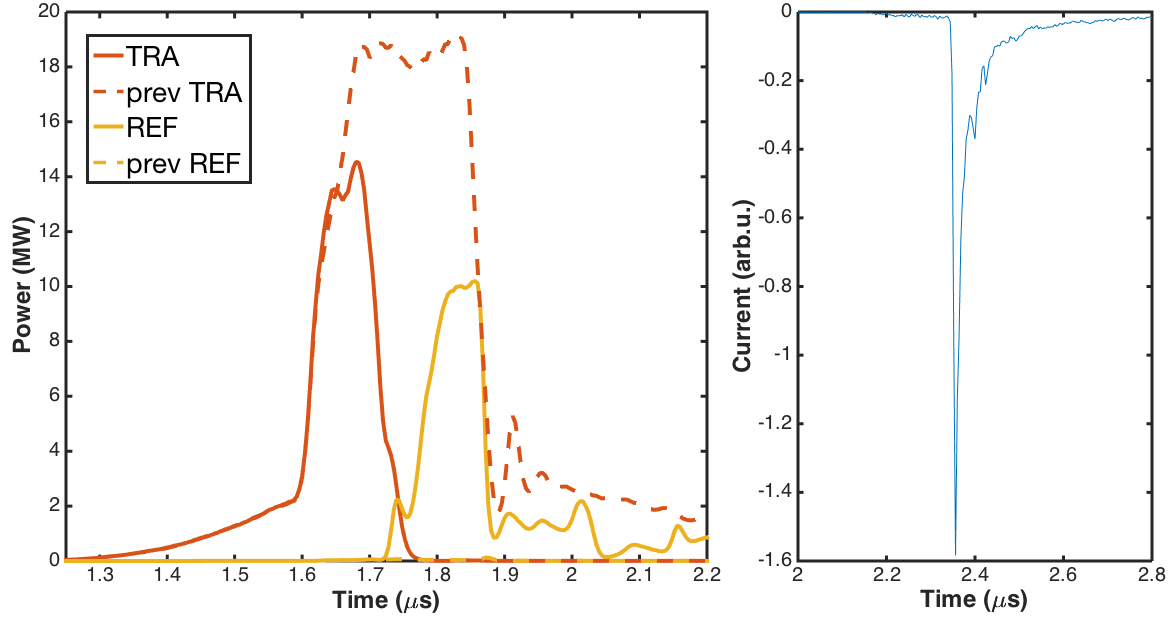
\includegraphics[scale=0.33]{pictures/RFandBPM.png}
\caption{RF signals during a breakdown (left) and burst of current emitted, detected by a BPM (right). In the left plot it is clearly visible the fall of the transmitted power (solid red) and the raise of the reflected power (solid yellow). The signals of the previous pulse, so without breakdown, are reported dashed. Note that the time scale in the two plots is not the same. Data acquired with the setup used in this work.}
\label{RFandBPM}
\end{figure}



\section[Vacuum arc process description]{Vacuum arc process description}

A fully satisfactory theory to describe the breakdowns has not been formulated yet, but the scientific community produced a number of models to describe the breakdown mechanism and initiation \cite{davies:triggers}. Most of them converge on the role that the field emission would have in triggering the breakdown, even if inconfutabile evidences have to be shown yet.

\subsection[Triggers]{Triggers}

The surface of the cathode is not completely flat, but presents some asperities that enhance the field emission as pointed out in chapter 2. This process leads to the formation of hot zones called \textit{field emitters} where the local electric field is enhanced of a factor $\beta$ because of the geometry and the current emitted is therefore increased (see figure \ref{BD_rocess}, box a). 

The current flow through the tip heats it up, modifying its physical properties and applying a tensile stress. Theories diverge on the process that takes place at this point: some prepend for the heating up of the tip up to the fusion, like \cite{Grudiev:newLoc}; others on the cracking process of the tip due to the tensile stress applied by the enhanced electric field, which gets comparable to the tensile strength of the material around $10$ GV/m  \cite{Insepov:1373092}.

It is in any case possible that during this process the shape of the tip gets modified, enhancing the $\beta$ factor even more.


\subsection[Plasma initiation]{Plasma initiation}

The peculiarity of the breakdown is that is a phenomenon that takes place in vacuum, and has been detected even at large gaps. According to many experimental results, the plasma is created from the cathode material (regardless on how it got emitted from the surface). The cathode material form a neutral gas surrounding the tip, that gets ionised by the electrons emitted by field emission (see figure \ref{BD_rocess}, box b). In this first phase the ions created in this manner drift under the effect of the space-charge effect. The plasma initiation last only few ns.

Spectroscopical measurements of the light emitted by the plasma flare have shown that the plasma is formed of ions with various charge and electrons. The DC spark system at CERN showed that the plasma formed by copper cathodes present ionisation levels up to Cu$^{3+}$. \cite{find quote}


\subsection[Plasma evolution]{Plasma evolution}

The ion density of the plasma over the emitter result in the establishment of a sheath potential, which enhances the electrical field, provoking an exponential  increase of the field-emitted current. The current emitted reaches values of several A/$\mu$m$^2$, determining the melting of the emitter (see figure \ref{BD_rocess}, box c).

The molten metal becomes part of the plasma, that expands modifying temperature and density. The sheath potential gets modified as well. After an expansion process, where part of the plasma interact with the surface, determining erosion, the greatest part of the ions recombinate with the electrons determining an intense optical emission.


\subsection[Cratering phase]{Cratering phase}

During the last plasma expansion, the ions impacting on the surface are expected to create new field emitters. The emitters will melt and result in an explosive emission because of the high field provoked by the sheath potential (see figure \ref{BD_rocess}, box d). 

The full arc is expected to continue up to the end of the RF pulse. Next the plasma is expected to disappear for expansion cooling or recombination. All the process result in a surface damage in the emitter zone and the surroundings. If in the damaged zone other asperities have been created, them will trigger new breakdowns according to the new value of $\beta$ (see figure \ref{BD_rocess}, box e, f). 

In figure \ref{SEM_crater} a photograph of a crater is shown, taken using a scanning emission microscope.
\begin{figure}[h]
\centering
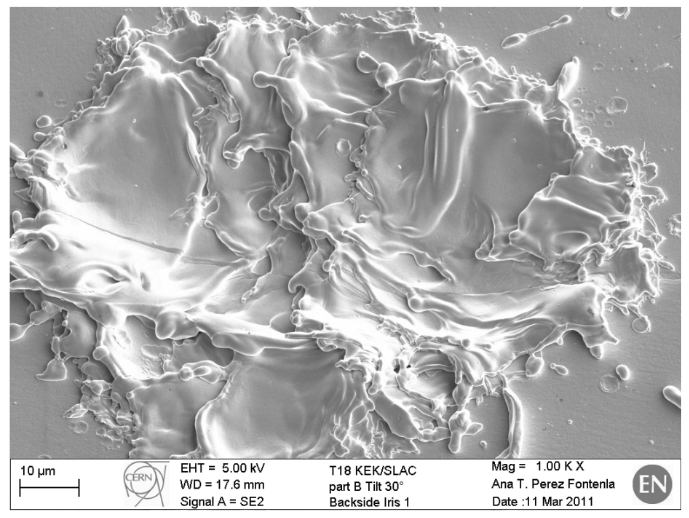
\includegraphics[scale=0.4]{pictures/crater}
\caption{Crater provoked by a breakdown in an X-band RF accelerating cavity \cite{Wuensch:advaces}}
\label{SEM_crater}
\end{figure}
Another review about the breakdown mechanism is \cite{soviet:1983}.




\begin{figure}[h]
\centering
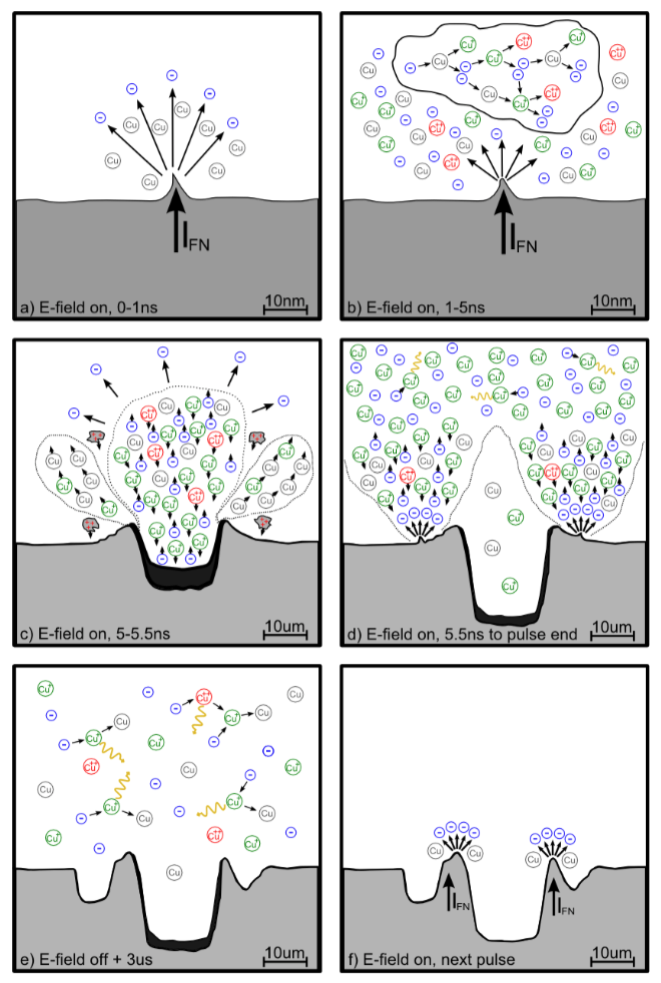
\includegraphics[scale=0.6]{pictures/BD_process}
\caption{Breakdown stages in chronological order. From \cite{Kovermann:1330346}}
\label{BD_rocess}
\end{figure}


\section[Influence of the conditioning process]{Influence of the conditioning process}























